\documentclass[letterpaper,12pt]{article}
\usepackage{lipsum}  
\usepackage{graphicx}
\usepackage{subcaption}
\usepackage[english]{babel}
\usepackage{fancyhdr}
\usepackage{outlines}
\usepackage{hyperref}
\usepackage[utf8]{inputenc} 
\usepackage{listings}
\usepackage{color}
 
\definecolor{codegreen}{rgb}{0,0.6,0}
\definecolor{codegray}{rgb}{0.5,0.5,0.5}
\definecolor{codepurple}{rgb}{0.58,0,0.82}
\definecolor{backcolour}{rgb}{0.95,0.95,0.92}

\lstdefinestyle{mystyle}{
    backgroundcolor=\color{backcolour},   
    commentstyle=\color{codegreen},
    keywordstyle=\color{magenta},
    numberstyle=\tiny\color{codegray},
    stringstyle=\color{codepurple},
    basicstyle=\footnotesize,
    breakatwhitespace=false,         
    breaklines=true,                 
    captionpos=b,                    
    keepspaces=true,                 
    numbers=left,                    
    numbersep=5pt,                  
    showspaces=false,                
    showstringspaces=false,
    showtabs=false,                  
    tabsize=2
}

\lstset{style=mystyle}

\graphicspath {{figures/}}

\setlength{\headheight}{15pt}

\pagestyle{fancy}
\fancyhf{}
\lhead{\textbf{Version:} 1  \textbf{Revision:} \today}
\rhead{\thepage}
\lfoot{Cole Kampa}
\rfoot{\textit{Mu2e: University of Minnesota}}

\renewcommand{\footrulewidth}{1pt}


\begin{document}
\begin{titlepage}
	\centering
	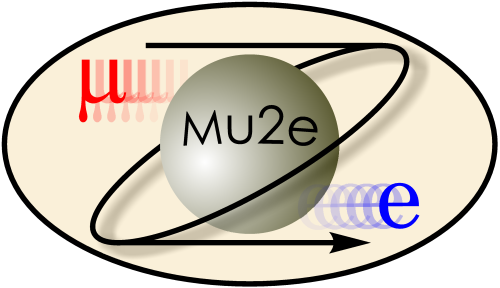
\includegraphics[width=0.5\textwidth]{mu2e_logo_oval.png}\par\vspace{2cm}
	{\scshape\LARGE Automated Sense Wire Tensioner: \\ Project Status Update 2\par}
	\vspace{3cm}
	{\Large Cole Kampa\par}
	%\vspace{3cm}
	\vspace{3.5cm}
	{\large University of Minnesota\par}
 	\vspace{.5cm}
	{\large \today \par}
	% Bottom of the page
	\vfill
	{kampa041@umn.edu\par}
\end{titlepage}

\clearpage
\setcounter{page}{2}


%actuator mount subfigure
\begin{figure}[h]
\centering
\begin{subfigure}{.5\textwidth}
  \centering
  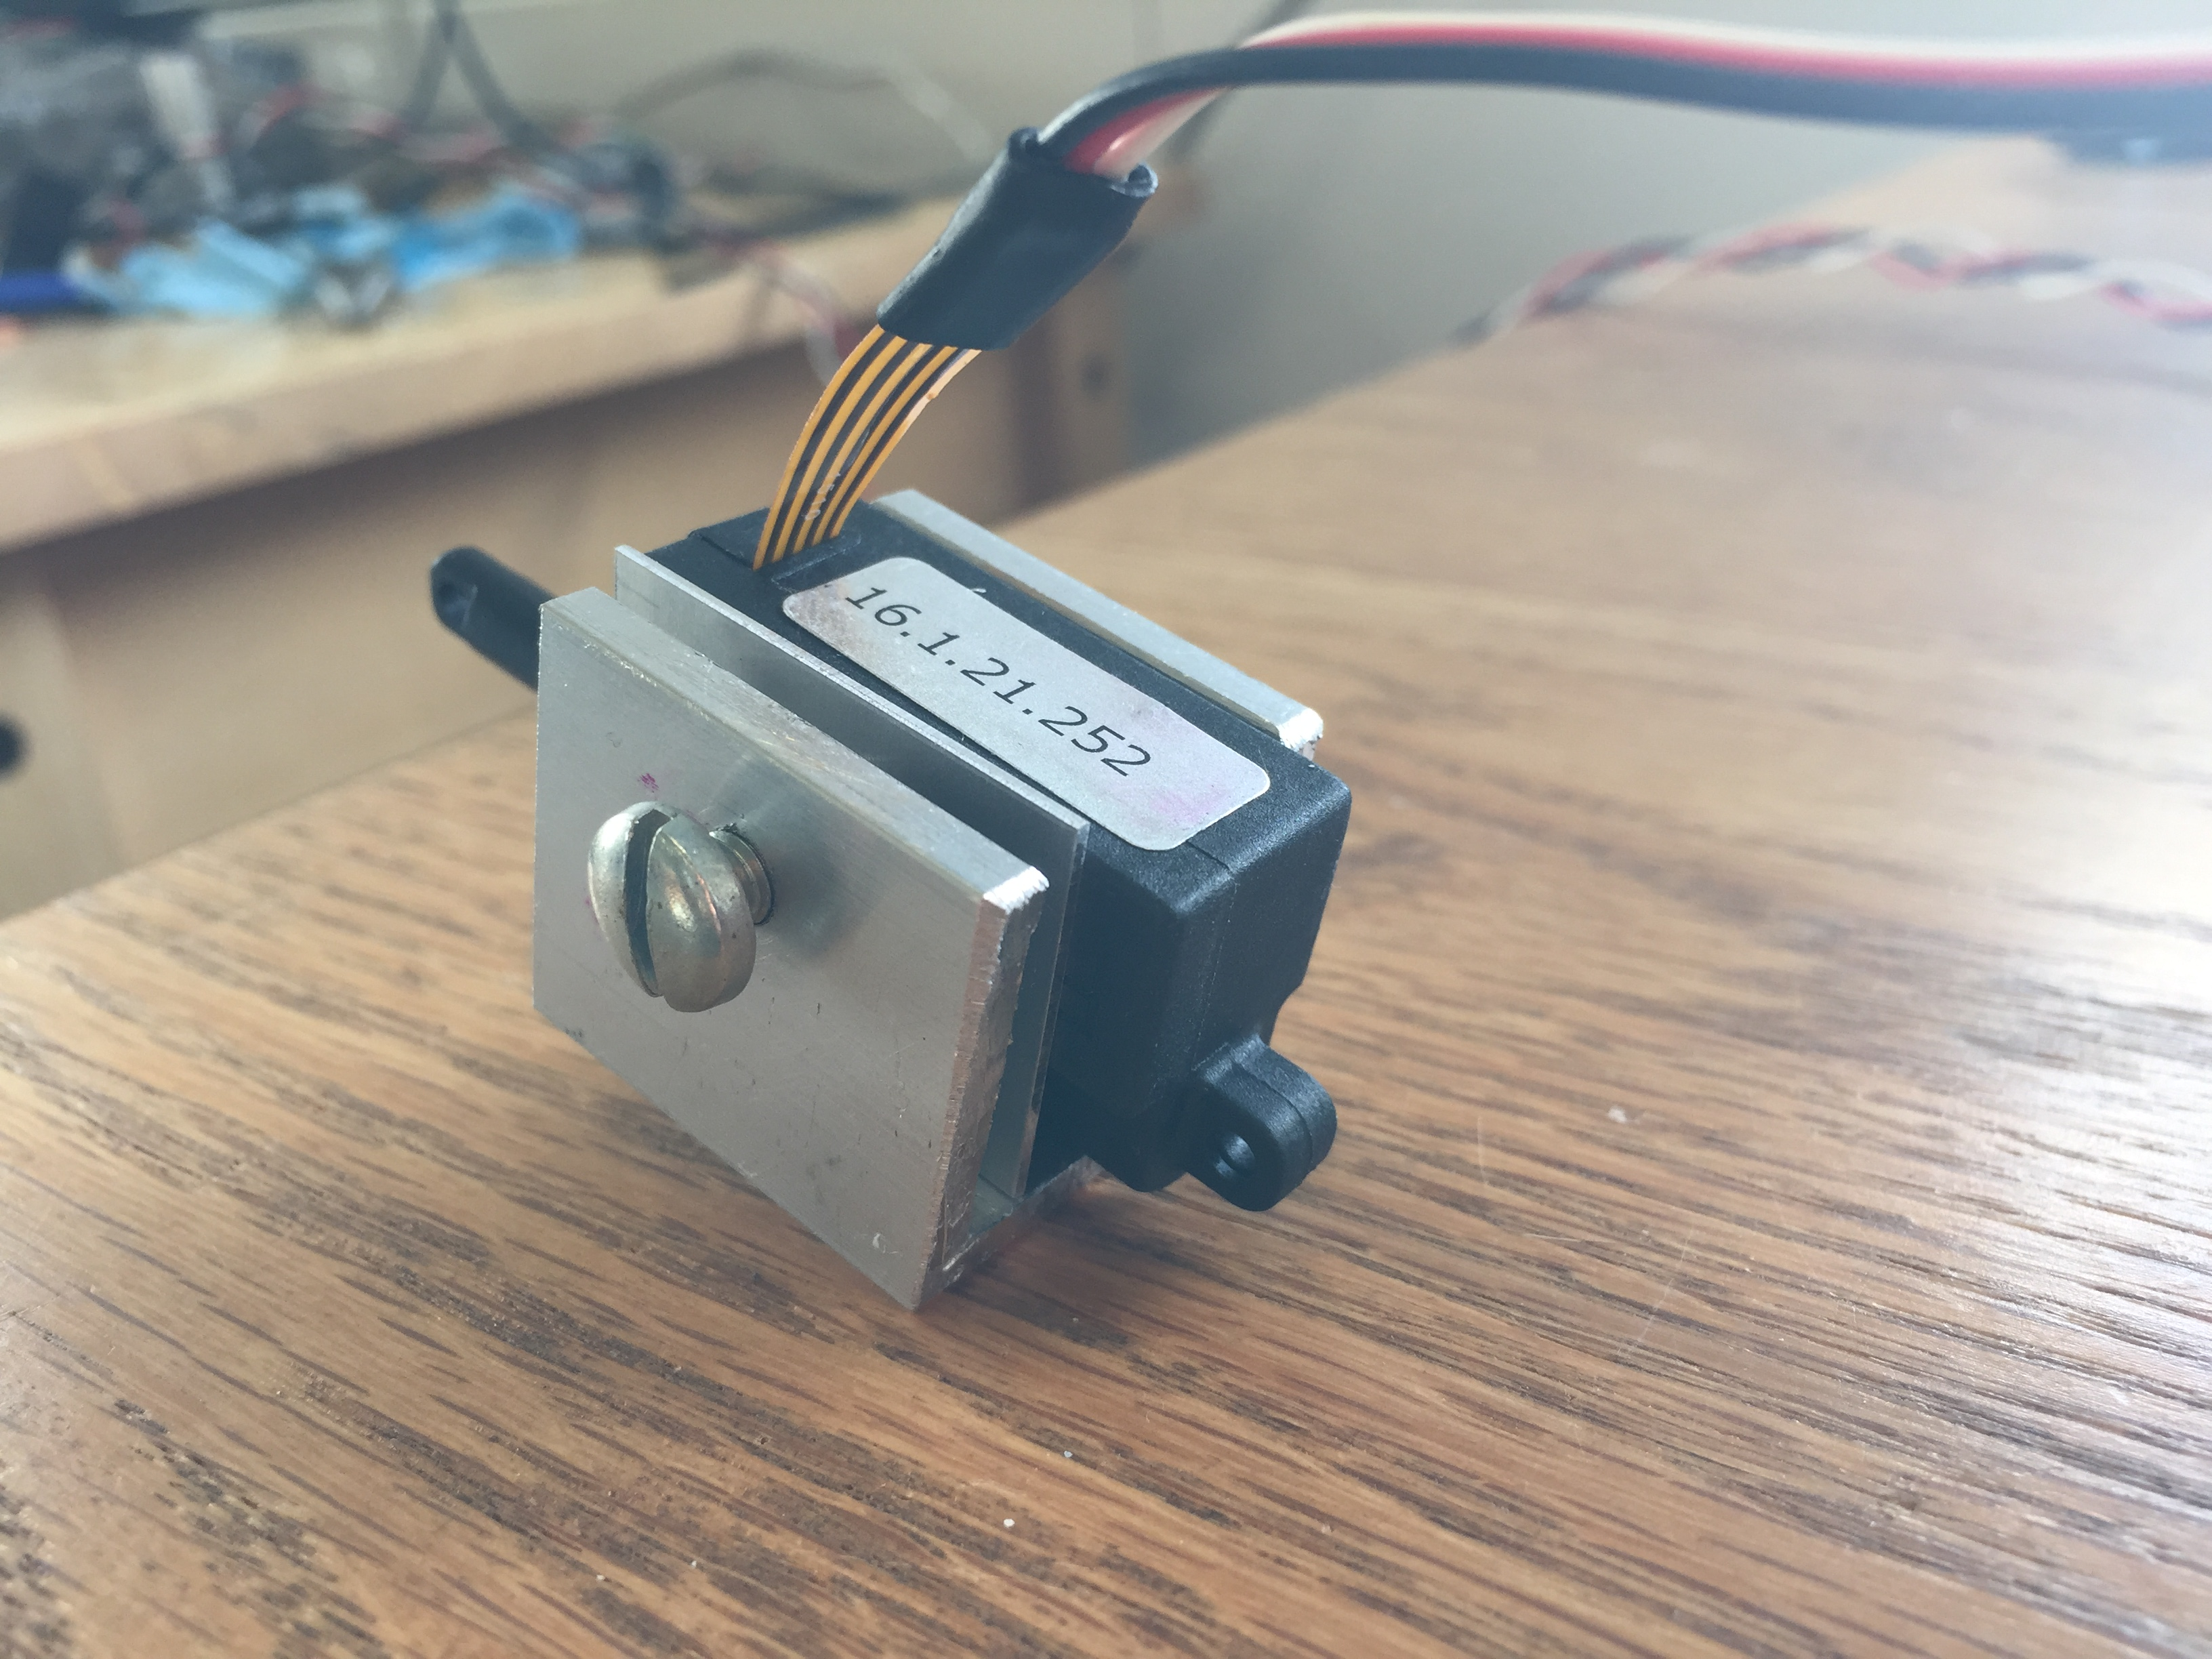
\includegraphics[width=0.9\linewidth]{actuator_mount.jpg}
\end{subfigure}%
\begin{subfigure}{.5\textwidth}
  \centering
  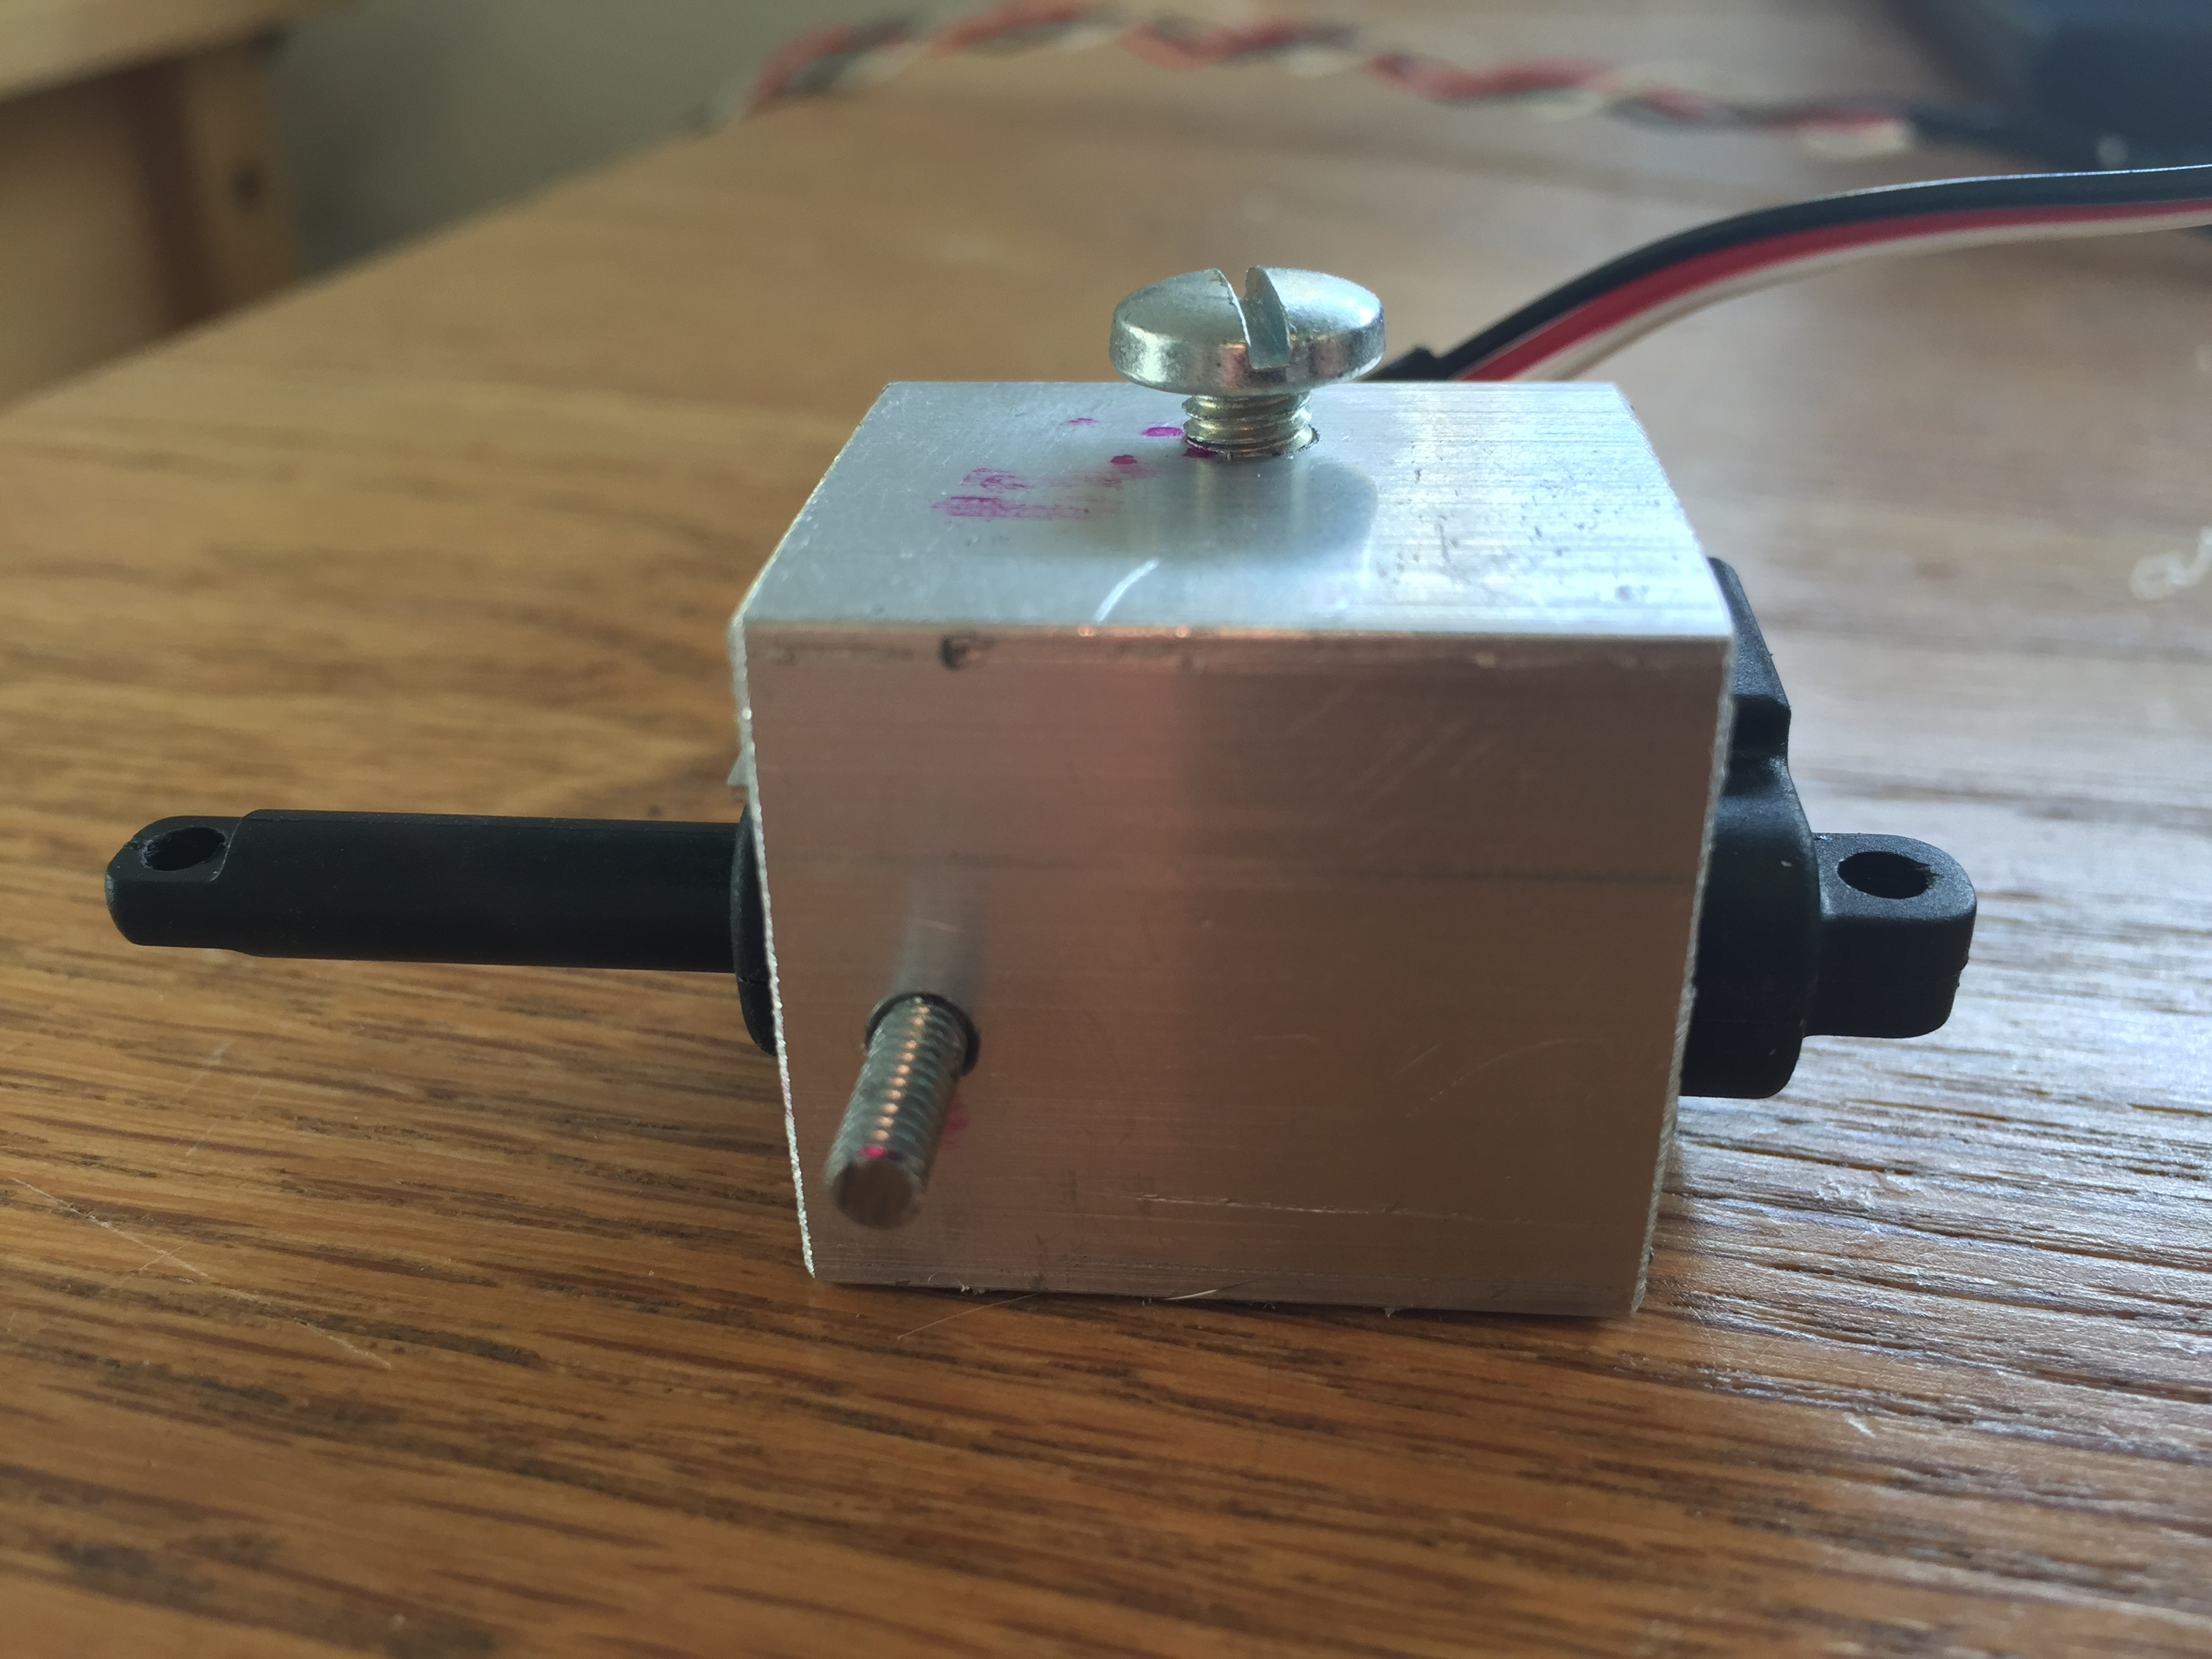
\includegraphics[width=0.9\linewidth]{actuator_mount_bottom.jpg}
\end{subfigure}
\caption{A U-channel piece of aluminum houses the actuator. A set screw tightens a thin sheet metal plate against the actuator. A screw is threaded through the bottom in place of a dowel pin (right).}
\label{fig:actuator}
\end{figure}

%load cell
\begin{figure} [h]
		\centering
		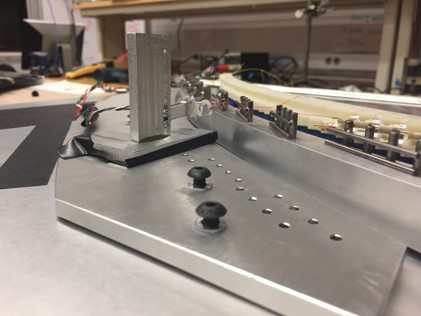
\includegraphics[width=1\textwidth,angle=0]{load_cell_mount.jpg}
		\caption{The load cell is fastened on one end to an aluminum upright epoxied with DP-810 to the aluminum base. A screw is used in place of a dowel pin. The screw fits into the positioning holes on the pulley plate.}
		\label{fig:load}
\end{figure}

%panel test
\begin{figure} [h]
		\centering
		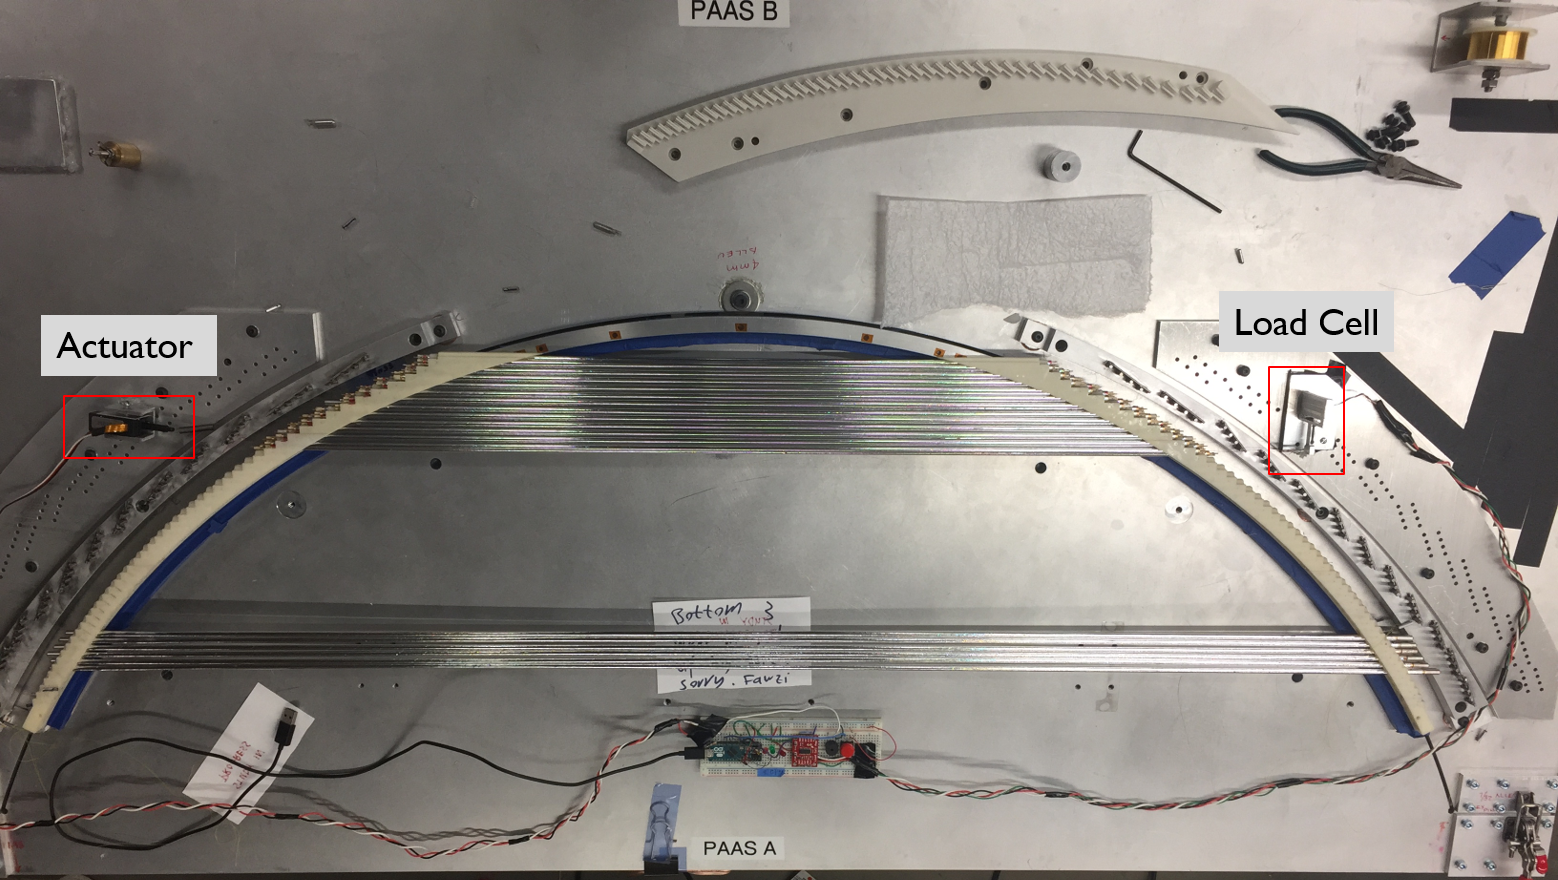
\includegraphics[width=1\textwidth,angle=0]{full_test_1.png}
		\caption{Setup of the first panel test for ergonomics of tensioning.}
		\label{fig:panel}
\end{figure}

%alligator clip subfigure
\begin{figure}[h]
\centering
\begin{subfigure}{.5\textwidth}
  \centering
  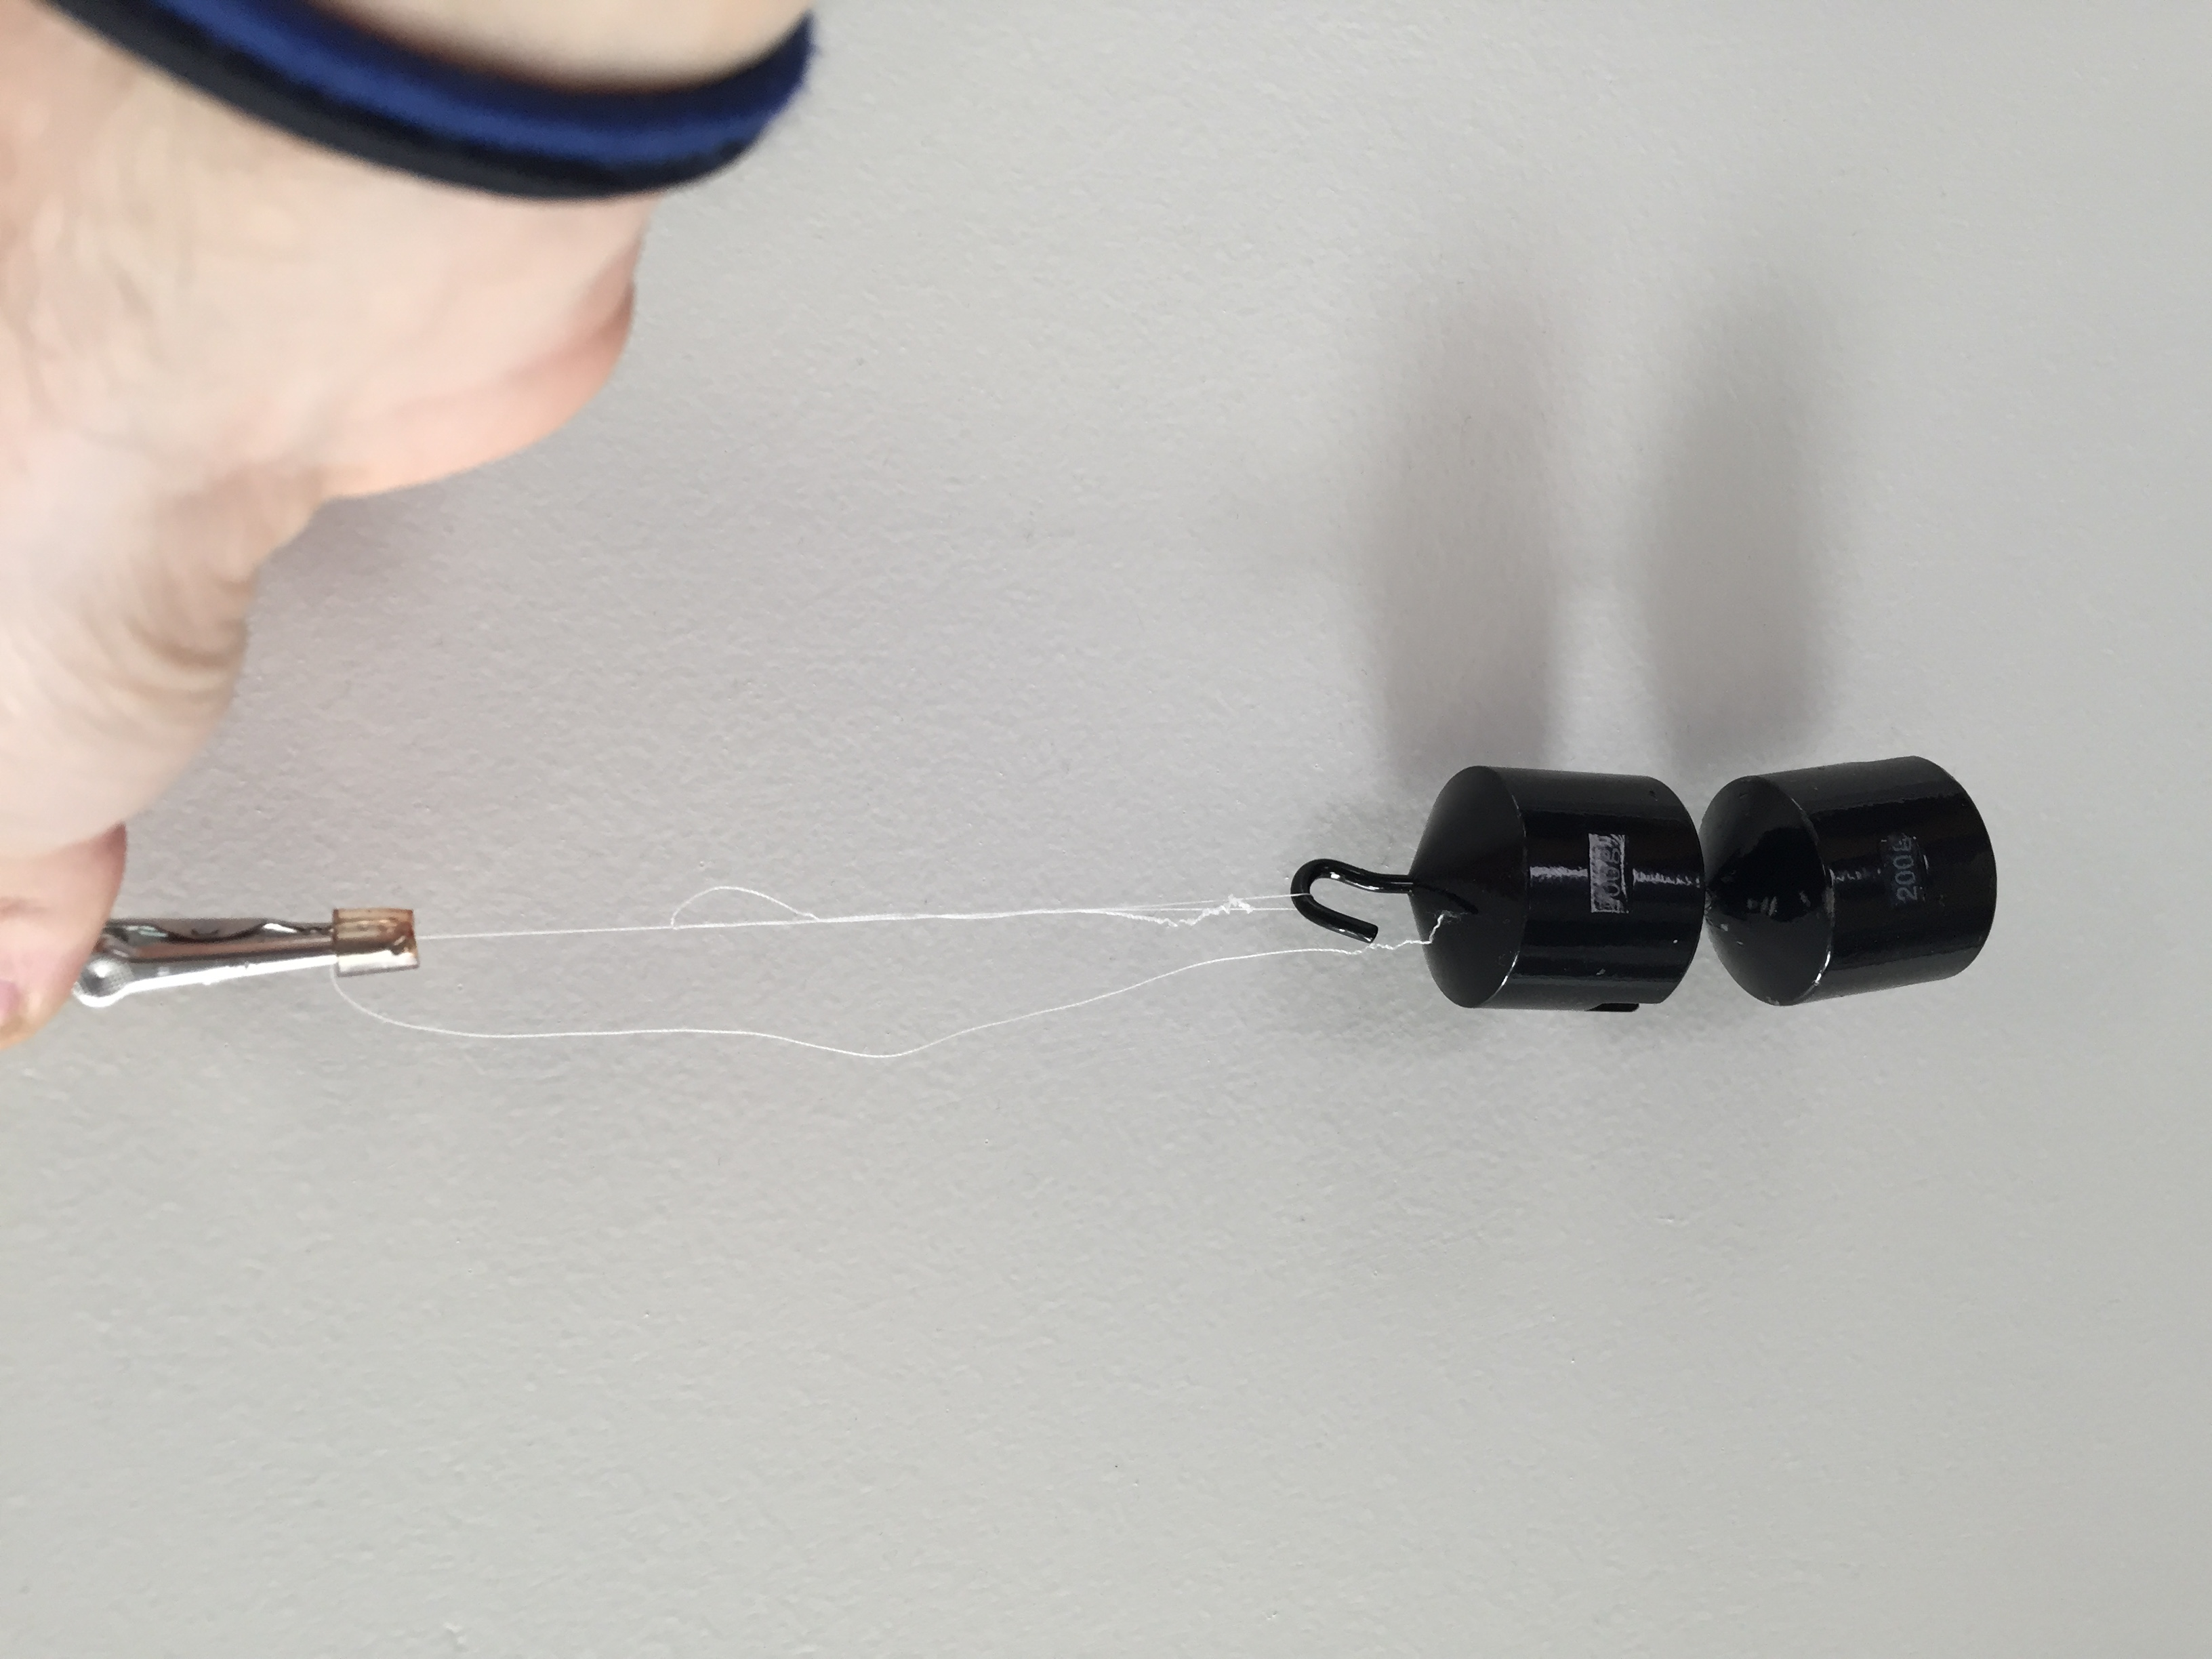
\includegraphics[width=0.9\linewidth, angle = -90]{thread_hold.jpg}
\end{subfigure}%
\begin{subfigure}{.5\textwidth}
  \centering
  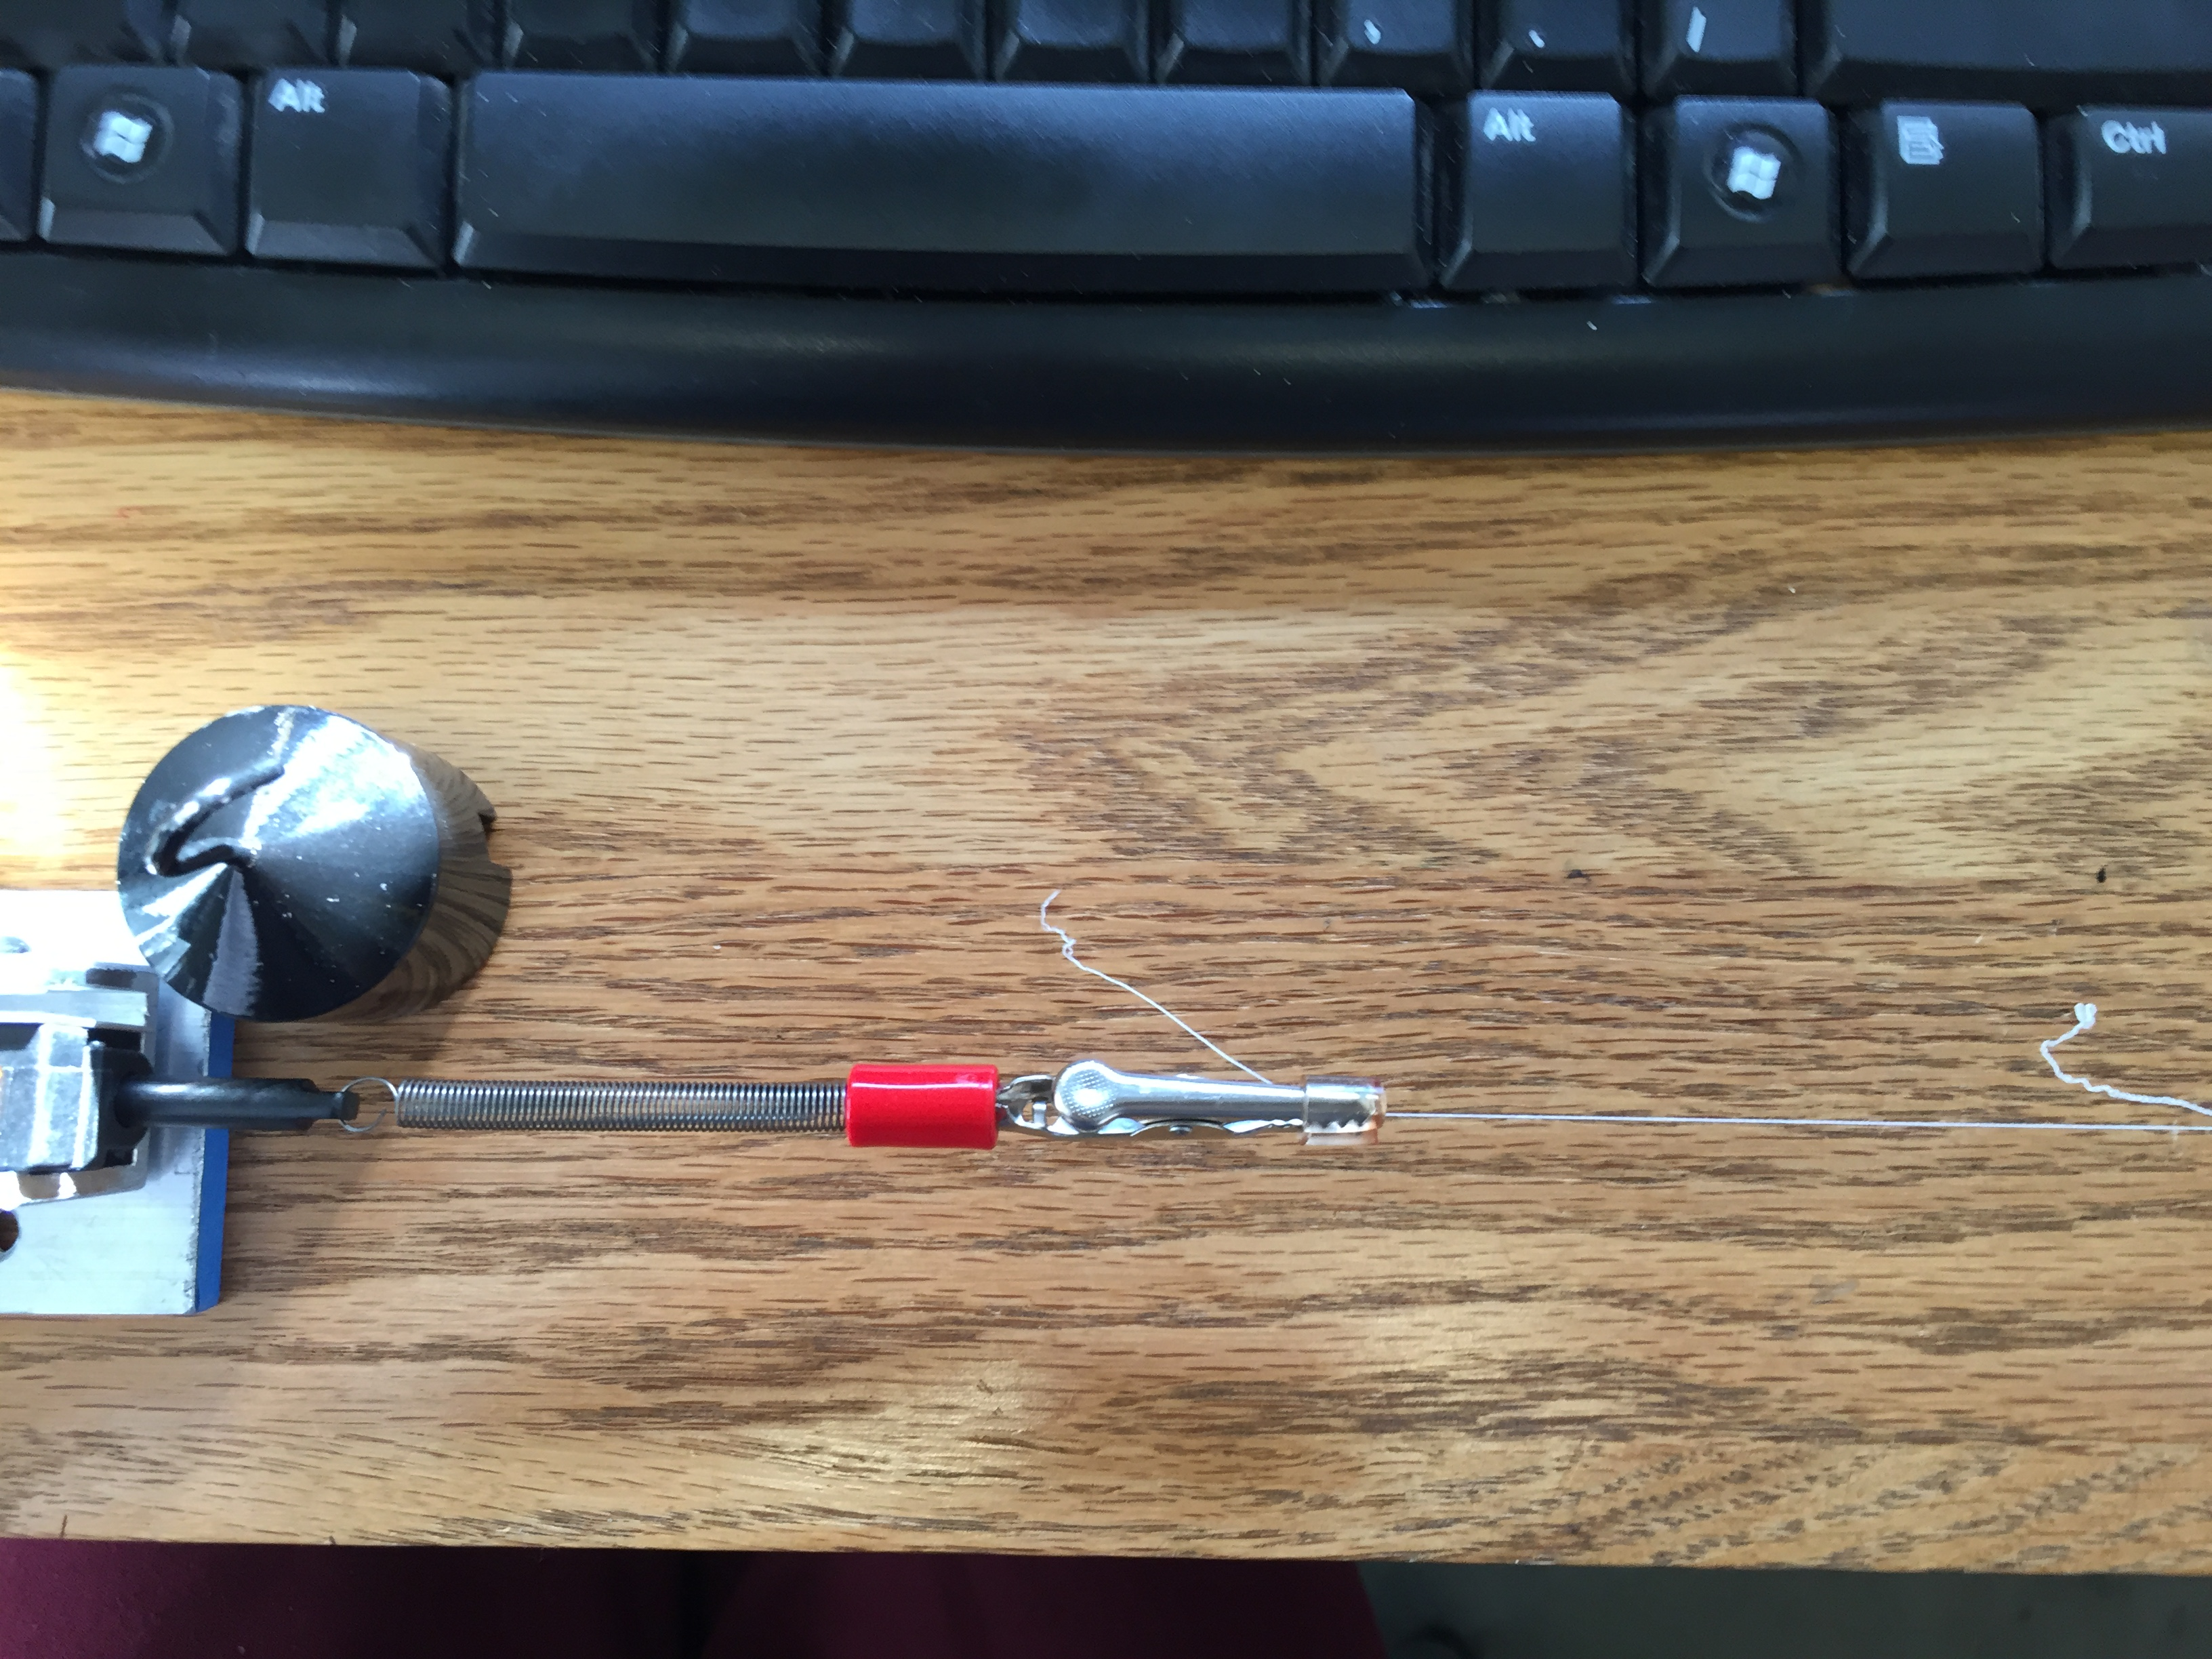
\includegraphics[width=0.9\linewidth]{alligator_motor.jpg}
\end{subfigure}
\caption{An alligator clip with protective tubing on the jaws can hold the thread up to 400 gf (left). Further designs must be made to attach the clip to the motor (right).}
\label{fig:thread}
\end{figure}

\section*{Recent Updates}
\begin{itemize}
\item{\textbf{Motor and Load Cell Mounts:} Finished prototype mounts for actuator (figure~\ref{fig:actuator}) and load cell (figure~\ref{fig:load}).}
\item{\textbf{First Panel Test:} Tested tensioning a thread with the test panel using the existing pulley plate holes (setup shown in figure~\ref{fig:panel}).
}
\item{\textbf{Planned Motor Replacement:} Switching the current motor to a more precise stepper motor should allow us to remove the weak spring and maintain a desired precision, which will simplify positioning (spring may sag). New motors and drivers have been ordered (1 week lead time).
}
\item{\textbf{Thread Gripping Method:} An alligator clip with the protective tubing still on the ends can grip the thread enough to hold up to 400gf (figure~\ref{fig:thread}). This is a quicker attachment than the previous loop and hot glue method. When the stepper motor arrives, we will have to find a way to fix the alligator clip to the linear motion piece of the motor.
}
\end{itemize}


\section*{To-Do}
\begin{outline}
  \1 Aruino Code:
    \2 Integrate the new stepper motor (\href{http://www.portescap.com/products/can-stack-linear-actuators/20dam-k-can-stack-stepper-linear-actuator}{20DAM10D1B-K}) + stepper driver (\href{https://www.digikey.com/product-detail/en/sparkfun-electronics/ROB-12779/1568-1108-ND/5318750?WT.srch=1&gclid=EAIaIQobChMI7vjsvPjX2QIVFiSBCh3bjw2JEAQYASABEgIDnfD_BwE}{ROB-12779}) [3 of each ordered on 3/7/18, send one set to Aseet at FNAL]
      \3 Find proper Arduino library for steppers and work to find the best way to control the stepper (feed in number of steps and speed)
      \3 A startup method must be in place to send the stepper back to a desired initial position. This will happen anytime the Arduino is reset.
    \2 Add calibration to main script for scheduled calibrations without changing the code
      \3 Can follow example in \texttt{SparkFun\char`_HX711\char`_Calibration} script i.e. calculate tension with current calibration factor, iterate with a conditional to adjust calibration factor until proper calculated tension is met.
    \2 Adjust peripherals (LEDs, Buzzer)
      \3 Right now, light indicates good or bad tension but LEDs are dim. Three buzzes if 80gf is never met. Add a long buzz for ``ready to solder ``.
    \2 Do not allow motor to oscillate about 80gf.
      \3 Because of the hysteresis in the sense wire, we want to pull to tension but never release the tension
  \1 Hardware:
    \2 Design mounts for load cell \& stepper motor with two dowel pins (two will help set the rotational position of the load cell and motor for accurate tension measurements)
      \3 Should make drawings to have these machined
      \3 The pulley plates will need to be adjusted to suit the second hole at each position. There is room to move the holes farther from comb if more space is needed.
    \2 Thread and wire holding methods
      \3 The thread can be held by alligator clips with protective plastic sleeves. Now we just have to find a way to mount the clip to the motor (see figure~\ref{fig:thread}).
      \3 Wire should be fixed to load cell end. No testing has been done with the alligator clips. The current method involves clamping the wire with a strong spring fixed to PAAS B. 
\end{outline}


\section{Arduino Code}
The following code ({\tt sense\_wire\_tension\_v2\_0.ino}) is currently being used.
\lstinputlisting[language=C++]{arduino_code/sense_wire_tension_v2_0/sense_wire_tension_v2_0.ino}


\end{document}